%  LaTeX support: latex@mdpi.com 
%  For support, please attach all files needed for compiling as well as the log file, and specify your operating system, LaTeX version, and LaTeX editor.

%=================================================================
\documentclass[journal,article,submit,pdftex,moreauthors]{Definitions/mdpi} 
%=================================================================
% MDPI internal commands - do not modify
\firstpage{1} 
\makeatletter 
\setcounter{page}{\@firstpage} 
\makeatother
\pubvolume{1}
\issuenum{1}
\articlenumber{0}
\pubyear{2025}
\copyrightyear{2025}
\datereceived{ } 
\daterevised{ }
\dateaccepted{ } 
\datepublished{ } 
\hreflink{https://doi.org/}

\usepackage{booktabs}
\usepackage{multirow}
\usepackage{graphicx}
\usepackage{xcolor}

% Full title of the paper (Capitalized)
\Title{AI Diffusion Model-Based Technology for Automating the Multi-Class Labeling of Electron Microscopy Datasets of Brain Cell Organelles for Their Augmentation and Synthetic Generation}

% MDPI internal command: Title for citation in the left column
\TitleCitation{Title}

% Author Orchid ID: enter ID or remove command
\newcommand{\orcidauthorA}{0000-0000-0000-000X}

% Authors, for the paper (add full first names)
\Author{Nikolay Sokolov \orcidA{}, Alexandra Getmanskaya \orcidA{} and Vadim Turlapov $^*$\orcidA{}}

% MDPI internal command: Authors, for metadata in PDF
\AuthorNames{Firstname Lastname, Firstname Lastname and Firstname Lastname}

\isAPAStyle{%
    				\AuthorCitation{Lastname, F., Lastname, F., \& Lastname, F.}
      			}{%
        \isChicagoStyle{%
        \AuthorCitation{Lastname, Firstname, Firstname Lastname, and Firstname Lastname.}
        }{
        \AuthorCitation{Lastname, F.; Lastname, F.; Lastname, F.}
        }
}

% Affiliations / Addresses (Add [1] after \address if there is only one affiliation.)
\address{\parbox{\textwidth}{Research Center for Artificial Intelligence, Institute of Information Technologies, Mathematics, and Mechanics, Lobachevsky University, 603022 Nizhny Novgorod, Russia; nikolay.sokolov@unn.ru (N.S.); alexandra.getmanskaya@itmm.unn.ru (A.G.)}}

% Contact information of the corresponding author
\corres{Correspondence: vadim.turlapov@itmm.unn.ru}

% Abstract (Do not insert blank lines, i.e. \\) 
\abstract{A technology for the automatic multi-class labeling of brain electron microscopy (EM) objects needed to create large synthetic datasets, which could be used for brain cell segmentation tasks, is proposed. The main research tools were a generative diffusion AI model and a U-Net-like segmentation model. The technology was studied on the segmentation task of up to six brain organelles. The initial dataset used was the popular EPFL dataset labeled for the mitochondria class, which has training and test parts having 165 layers each. Our mark up for the EPFL dataset was named EPFL6 and contained six classes. The technology was implemented and studied in a two-step experiment: (1) dataset synthesis using a diffusion model trained on EPFL6; (2) evaluation of the labeling accuracy of a multi-class synthetic dataset by the segmentation accuracy on the test part of EPFL6. It was found that (1) the segmentation accuracy of the mitochondria class for the diffusion synthetic datasets corresponded to the accuracy of the original ones; (2) augmentation via geometric synthetics provided a better accuracy for underrepresented classes; (3) the naturalization of geometric synthetics by the diffusion model yielded a positive effect; (4) due to the augmentation of the 165 layers of the original EPFL dataset with diffusion synthetics, it was possible to achieve and surpass the record accuracy of Dice = 0.948, which was achieved using 3D estimation in Hive-net (2021).}

% Keywords
\keyword{diffusion neural network; automatic multi-class labeling; electron microscopy; synthetic dataset; dataset augmentation; geometric augmentation; semantic segmentation}

\begin{document}

\section{Introduction}

As the title suggests, this article proposes a technology for the automatic multi-class labeling of brain electron microscopy (EM) objects based on a generative diffusion model. Despite the recent emergence of diffusion models, according to the review [1], many new methods for segmentation and diagnostics in biomedicine have already been developed based on them. But for the technology to emerge, it is also necessary to automate unlimited-volume synthetic EM dataset creation for training foundation models [2] to replicate technologies in downstream applications. Such technologies are also relevant for augmenting existing datasets. Specifically, the area of segmentation and classification of brain cell organelles based on brain EM data has many of its own features that complicate the problem. The complexity of this problem stems from the fact that EM operates at the limit of its resolution capabilities (units of nanometers) when capturing organelle images. This leads to a high level of noise in the images, significantly impacting the accuracy and feasibility of segmenting individual organelles. Another challenge is the significant variation in the representation of different organelles per unit area of the EM layer, as well as their underrepresentation in the dataset as a whole. The traditional solution of this problem is an augmentation of real data datasets using classical methods (reflection, rotation, tiling, etc.). This solution is simple and cost-effective but does not solve the problem completely. The development of neural networks, particularly generative models, has given rise to data augmentation (DA) methods leveraging these technologies. One of the earliest studies to use serial block scanning electron microscopy (EM) as a source of high-resolution three dimensional nanohistology for cells and tissues was ref. [3]. A subsequent series of works was aimed at creating datasets for training deep learning networks for EM data segmentation designed for the binary segmentation of brain cell organelles–neural membranes [4] and the supervoxel segmentation of mitochondria [5]. Simultaneously, the problem of 3D reconstruction of the brain neural network and the problem of brain connectomics on the basis of neuron organelles and connections between neurons (synapses) is stated in [6]. In this problem, of particular importance is the segmentation of postsynaptic densities (PSDs), vesicles, and axons.

The invention of U-Net in 2015 [7] gave rise to numerous novel models and adaptations for segmenting brain EM data. The reason for U-Net’s success is related to the contextual information of an input image at all levels of processing. Almost immediately, the publication [8] experimentally confirmed that the skip connection of the U-Net architecture is effective in solving segmentation problems in biomedicine.

U-Net also provided a basis for creating numerous models: [9,10], 3DU-Net [11], V-Net [12], DeepMedic [13], HighRes3DNet [14], Inception U-Net [15], R2U++ [16].

The application of artificial intelligence methods for EM data processing is significantly hindered by the limited availability of labeled data for training and testing deep neural networks (DNNs). Open EM data as a whole are represented by only a few labeled datasets, both due to the laboriousness of preparing samples for an electron microscope, and due to the lack of specialists for manual labeling. Labeling electron microscopy data remains a time-consuming and labor-intensive task, with the annotation of a single experiment requiring up to six months of manual effort. We found four open EM datasets, the earliest and most popular of which were only labeled for one class (mitochondria or membranes). In the two other datasets, several classes were distinguished. As a result, the majority of neural networks used in EM processing are only trained to perform binary segmentation.

According to articles by [17 ,18], DA is a recognized effective solution to expand the training dataset. The cheapest and most effective of the traditional augmentation methods are horizontal and vertical flipping, translation, and cropping. This means that the relative arrangement of the compartments remains unchanged. With the development of neural networks, there is now the possibility of using deep learning models to generate synthetic images for DA goals.

One of the popular solutions was the use of Generative Adversarial Networks (GANs) [19–22] to augment data for classes that are underrepresented in the dataset. Employing GANs for data generation [23] can yield images practically indistinguishable from real ones. However, training these neural networks requires a large volume of data, and this process may be unstable [24].

However, despite the simplicity of classical augmentation methods, according to a study [25] on the classification task, cropping is more effective than WGAN.

Using variational autoencoders (VAEs) [26] enables training on unlabeled data; however, the quality of generation may be inferior to real data.

Neural diffusion (ND) models are an advanced approach in the field of artificial intelligence that models information diffusion in neural networks to achieve realistic results. They define a Markov chain of diffusion steps to gradually add random noise to the data and then learn to reverse the diffusion process to generate desired data samples from the noise. This method finds widespread application in generative modeling, texture synthesis, and image restoration [ 27 ]. Recently, the probabilistic model of diffusion denoising (DDPM) [ 28 ] has garnered significant attention due to its excellent quality in generating synthetic images [24,29,30].

The main advantages of neural diffusion (ND) models can be summarized as follows:
\begin{enumerate}
	\item {ND enables the generation of high-quality images with rich details, realistic textures,
	and smooth transitions. This approach is capable of eliminating noise and artifacts,
	resulting in the generation of clean and natural images.} 
	\item {The ND approach provides control over the image generation process. Through
	diffusion parameters, one can adjust the level of detail and blur or the degree of
	preserving the original information. This allows users to customize generated images
	according to specific requirements.}
	\item	{ND can be applied to various types of images, including photographs, drawings, textures,
	and others. This makes it a versatile tool for generating and processing diverse kinds of
	visual data.}
\end{enumerate}

The flexible DA method based on diffusion models proposed in ref. [31] outperforms the standard DA baseline by about 0.3 accuracy points for the classification task.

The achievements of expanding the dataset for the segmentation task are not so impressive. Ref. [32] proposed expanding the dataset using a diffusion neural network and improved the segmentation results by 0.01–0.03 values in the Dice metric.

The most interesting publication in recent years for us was a review [33] devoted to the study of the capabilities of diffusion models in medical problems. These tasks include anomaly detection; medical image segmentation; noise suppression; classification, generation, and others. Three main approaches to diffusion modeling are characterized as follows: Denoising Diffusion Probabilistic Models (DDPMs), Noise Conditioned Score Networks (NCSNs), and Stochastic Differential Equations (SDEs). The greatest attention is paid to the DDPM approach; so-far unresolved problems are also considered.

In our previous papers [34, 35], we considered the problem of recognition by neural networks of classes that are underrepresented in the training dataset. To achieve this, we proposed using a geometric parametric algorithm that allows us to create the required number of missing images and markings for them. This approach was effective, but the generated images lacked realism. The idea for the further development of this approach to augmentation was suggested by an article linking the modeling of nonequilibrium thermodynamics with modern diffusion models [36]. Such models are capable of turning any simple geometric models into realistic images with noise to the required degree.

Thus, the above review ultimately inspired us not only to explore the possibilities of diffusion neural network models that would provide the augmentation of real data simultaneously with their labeling, but also to increase the similarity of simple geometric models to real data, also through diffusion models.

Additionally, we aimed to develop and explore a multi-class technology for the automatic labeling of EM data, invariant to the number and diversity of organelles. This was demonstrated using six organelles as examples: mitochondria, mitochondria boundaries, vesicles, postsynaptic densities (PSDs), cell membranes, and axon sheaths (including their contents).

\section{Materials and Methods}
\subsection{Segmentation Task, Metric, and Network}

Semantic Segmentation is a computer vision task in which the goal is to produce a dense pixel-wise segmentation map of an image, where each pixel is assigned to a specific class or object.

We used the Dice–Sørensen coefficient (DSC, Dice), a metric commonly used for evaluating the segmentation of biomedical images. The DSC values ranged from zero to one. Let the number of pixels correctly classified as belonging to the target class be defined as the true positive (TP), the number of correctly classified background pixels as the true negative (TN), the number of pixels erroneously classified as belonging to the target class as the false positive (FP), and the number of erroneously classified background pixels as the false negative (FN). The DSC metric is then defined as follows:

This is the example 1 of equation:
\begin{equation}
DSC = \frac{2TP}{2TP+FP+FN}
\end{equation}

Since we consider multi-class segmentation in this study, we are interested in multi-class evaluation metrics. Since the Dice metrics compare two sets, in the case of multi-class classification, the result will be a vector of Dice metrics for each class. For training a neural network for multi-class segmentation, we should transform DSCi metrics to the scalar error or loss function. For this purpose, we use the linear combination defined in Equation (2):

\begin{equation}
Loss = \alpha _i\sum_{i = 1}^{N}\alpha _i (1-DSC_i),\alpha _i \geq 0,\sum_{i = 1}^{N}=1
\end{equation}

where Loss is a scalar total multi-class loss function, N is the number of classes, $\alpha _i$ is a weighting coefficient, and $\mathcal(1 - DSC_i)$ is the loss value for the i-th class. The weight coefficients $\alpha _i$ were chosen equal to 1/N.

\vspace{10pt}
\noindent {Segmentation Network Architecture}

U-Net is widely regarded as a standard convolutional neural network architecture for biomedical image segmentation tasks. The architecture comprises two main components: a contracting path, which captures global context and feature hierarchies, and a symmetric expanding path, which enables precise localization of structures. The basis of the network of our study is the U-Net project (\href{https://github.com/zhixuhao/unet}{https://github.com/zhixuhao/unet}, accessed on 2 December 2024). In the original project, U-Net was used for the binary classification of membranes.

We built compact modifications of the U-Net model and present here the tiny-U-Net model. The architecture of our simplified model is illustrated in Figure 1.

The tiny-U-Net has the following differences from the previous architecture:
\begin{itemize}
	\item {Our network input is an image of size 256 × 256 × 1 instead of 512 × 512 × 1.}
	\item {Our network output is 256 × 256 × N instead of 512 × 512 × 1, where N is the number of classes.}
	\item {We added batch normalization after each ReLU, convolution, and activation layers.}
	\item {Number of channels in the original U-Net convolution blocks: 64 → 128 → 256 → 512 → 1024; number of channels in our architecture: 32 → 32 → 64 → 128 → 256}
	\item {The resulting model contains 15.7 times fewer parameters than the original model and takes up 15.2 times less memory (24 MB instead of 364 MB)}
\end{itemize}

As in the original project, we use the output activation function sigmoid. We extend the application of this function not only for binary but also for multi-class segmentation. Using this activation function guarantees that each mask is in the range of [0, 1] and also provides the independence of masks. In this approach, one pixel of the layer can be associated with several classes at once, unlike the standard approach with the softmax function.

\begin{figure}[H]
	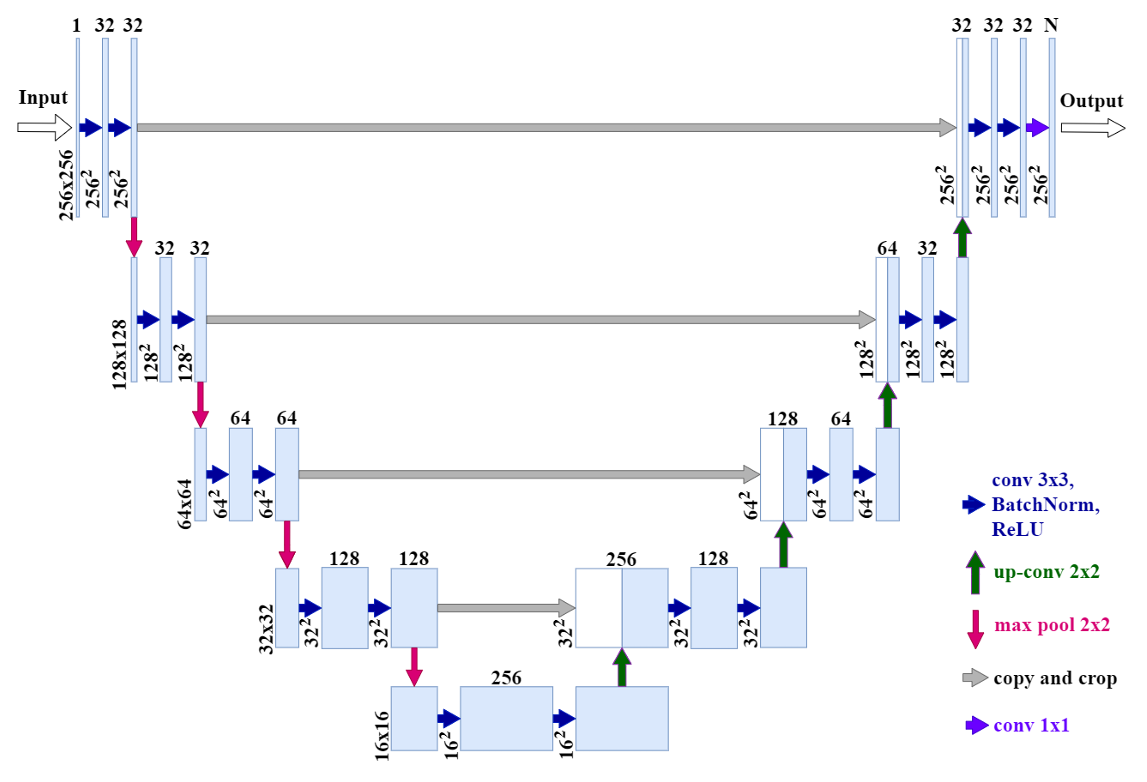
\includegraphics[width=12 cm]{Definitions/figure-1.png}
	\caption{he architecture of the tiny-U-Net model.\label{fig1}}
\end{figure}

\subsection{Datasets and Their Markups}
In this section, we provide an overview of publicly available datasets for electron microscopy (EM) segmentation task (Table 1). Among the most widely used datasets for this task are those collected by Lucchi et al. in [37]. These datasets have become a benchmark for evaluating segmentation performance in EM images.

\begin{table}[H] 
	\caption{Open labeled electron microscopy datasets.\label{tab1}}
	\begin{adjustwidth}{-\extralength}{0cm}
	\begin{tabularx}{\fulllength}{CCCCCC}
	\toprule
	\textbf{No.}	& \textbf{Name}	& \textbf{Data Volumes}	& \textbf{Labeled Data Volumes}	& \textbf{Labeled Classes}	& \textbf{Resolution (nm/voxel)}\\
	\midrule
	1		& AC4, ISBI 2013 [38]	& 4096 × 4096 × 1850 & 1024 × 1024 × 100 & membranes & 6 × 6 × 30\\
	\hline
	2		& EPFL \textsuperscript{b}, Lucchi++ \textsuperscript{c} [5] & 1065 × 2048 × 1536 &2 datasets, 1024 × 768 × 165 & mitochondria & 5 × 5 × 5\\
	\hline
	3		& Kasthuri et al. [39] & & 1334 × 1553 × 75 1463 × 1613 × 85 & mitochondria & 3 × 3 × 30\\
	\hline
	4		& UroCell \textsuperscript{a} [40] & 1366 × 1180 × 1056 & 5 datasets, 256 × 256 × 256 & mitochondria, endolysosomes, fusiform vesicles & 16 × 16 × 15\\
	\bottomrule
	\end{tabularx}
	\end{adjustwidth}
	
	\noindent{\footnotesize{\textsuperscript{a} Data are available on GitHub: https://github.com/MancaZerovnikMekuc/UroCell, accessed on 2 December
	2024.\textsuperscript{b} EPFL dataset is available at https://www.epfl.ch/labs/cvlab/data/data-em/, accessed on 2 December
	2024. \textsuperscript{c} Data are available at https://casser.io/connectomics/, accessed on 2 December 2024.}}
\end{table}

It is seen that in three of the four labeled open datasets, only one class is labeled. Only one dataset contains more than one labeled class. For this reason, the vast majority of neural networks in EM are trained to classify only two classes (object and background).

For our study, we utilized the EPFL dataset, which is publicly available at \url{https://www.epfl.ch/labs/cvlab/data/data-em/}, accessed on 2 December 2024. The data used in this work were acquired by a focused ion beam scanning electron microscope (FIB-SEM, Zeiss NVision40), which uses a focused beam of gallium ions to mill the surface of a sample and an electron beam to image the milled face. The milling process removes approximately 5 nm of the surface, while the scanning beam produces images with a pixel size of 5 × 5 nm [5]. This dataset comprises images obtained from the CA1 region of the hippocampus in the brain, with a voxel resolution of approximately 5 × 5 × 5 nm. The training set includes 165 image stack fragments, each with a size of 1024 × 768 pixels. This dataset was acquired by Graham Knott and Marco Cantoni at EPFL. Notably, the original EPFL dataset provides annotations exclusively for mitochondria. The test set of the EPFL dataset consists of 165 full-size images (1024 × 768 pixels) with corresponding ground truth annotations for mitochondria. These test images are used to evaluate the generalization capability of trained models on unseen data. An example of the dataset is illustrated in Figure 2.

\begin{figure}[H]
	\subfloat[\centering]{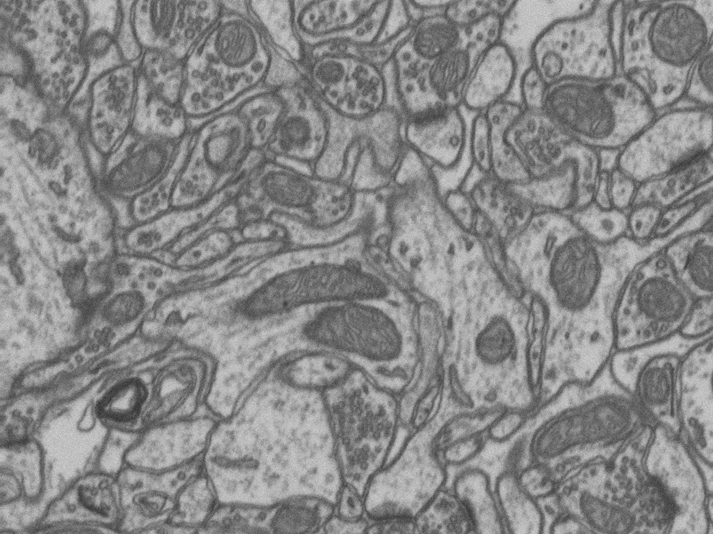
\includegraphics[width=4.5cm]{Definitions/figure-2a.png}}
	\hspace{0.2cm}
	\subfloat[\centering]{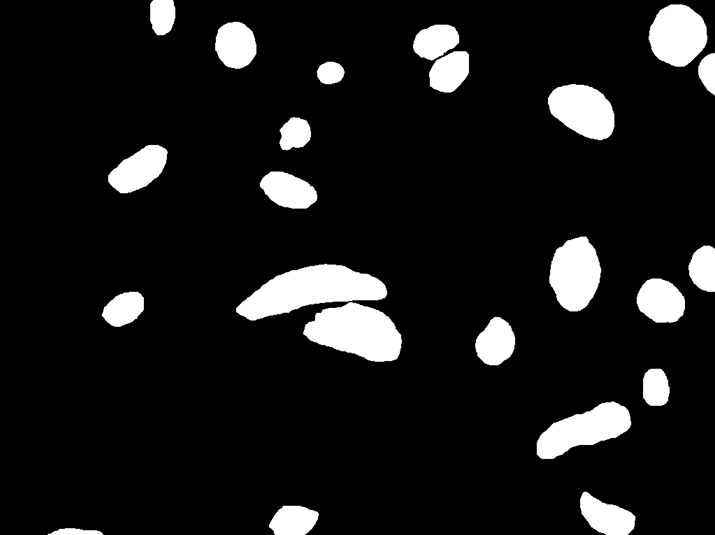
\includegraphics[width=4.5cm]{Definitions/figure-2b.png}}
	\caption{The electron microscopy 1024 × 768 image from the EPFL dataset of a mouse brain and mitochondrial annotation: (\textbf{a}) EPFL layer; (\textbf{b}) Annotation mask.\label{fig2}}
\end{figure}

For the EPFL dataset, an enhanced annotation called Lucchi++ is available [ 41 ]. The research team re-annotated two EPFL Hippocampus image stacks to enhance the consistency and accuracy of mitochondrial membrane labeling. The process involved a senior biologist manually refining the annotations, which were then independently reviewed by two neuroscientists. Disagreements were resolved through iterative corrections, ensuring consensus and high-quality annotations. In other words, the Lucchi++ dataset provided an enhanced labeling for both the training and test sets of the EPFL dataset, with each stack having dimensions of 165 × 1024 × 768 pixels.

But in addition to mitochondria, the EPFL dataset can be marked with 4 types of compartments: PSD, vesicles, membranes, and axons. And if the first three are presented in the dataset as well as mitochondria, axons, on the contrary, are very poorly represented. The axons’ sheath in the training dataset is present only in the first 36 layers and looks completely different from the axon sheath in the test dataset Figure 3. In the test dataset, axons appear in the first 70 layers, transitioning from an elongated to a more rounded shape. Additionally, they exhibit a darker interior and an inner ring, further distinguishing them from the training set.

\begin{figure}[H]
	\subfloat[\centering]{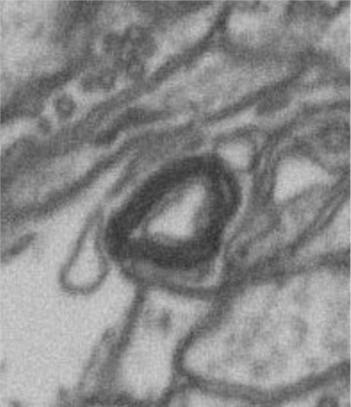
\includegraphics[width=2.5cm]{Definitions/figure-3a.png}}
	\hspace{0.1cm}
	\subfloat[\centering]{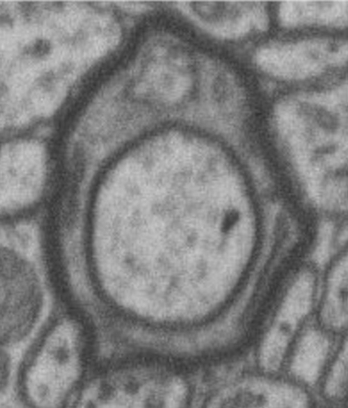
\includegraphics[width=2.5cm]{Definitions/figure-3b.png}}
	\hspace{0.1cm}
	\subfloat[\centering]{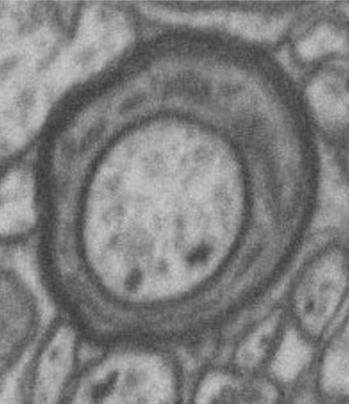
\includegraphics[width=2.5cm]{Definitions/figure-3c.png}}
	\hspace{0.1cm}
	\subfloat[\centering]{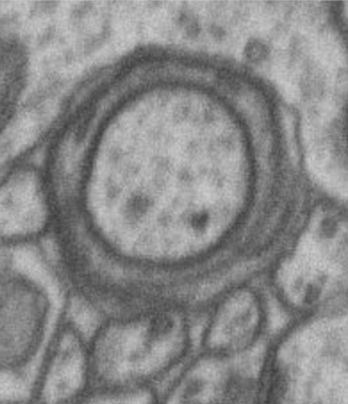
\includegraphics[width=2.5cm]{Definitions/figure-3d.png}}
	\caption{Axon sheath in the training and test EPFL datasets: (\textbf{a})  axon sheath in the training set; (\textbf{b}) axon sheath in the test set, first layer; (\textbf{c}) axon sheath in the test set, 35th layer; (\textbf{d}) axon sheath in the test set, 70th layer.\label{fig3}}
\end{figure}

Since we wanted to deal with multi-class segmentation, we had to make our own markup for the existing dataset [42]. We marked 55 training layers and 5 test ones, on which we tested multi-class models. Also, we tested our models on the full EPFL test volume and the complete Lucci++ markup to compare our results with other studies.

Thus, in our work, we used three markups of the same dataset (EPFL, Lucchi++, and ours markups); the difference between the markups is shown in the Figure 4. We calculated the differences between markups using the formula:

\begin{equation}
	difference = \frac{\textit{count\_different\_areas\_in\_pixels}}{\textit{count\_intersection\_in\_pixels}}
\end{equation}

\begin{figure}[H]
	\subfloat[\centering]{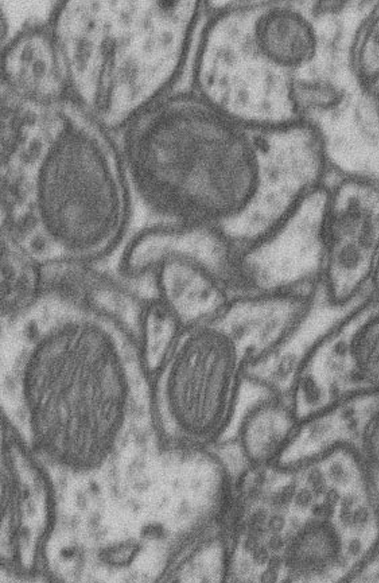
\includegraphics[width=2.5cm]{Definitions/figure-4a.png}}
	\hspace{0.1cm}
	\subfloat[\centering]{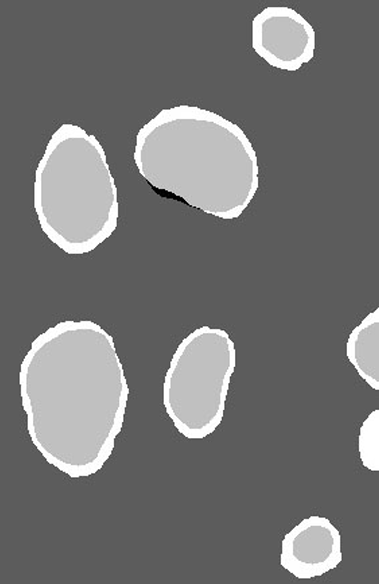
\includegraphics[width=2.5cm]{Definitions/figure-4b.png}}
	\hspace{0.1cm}
	\subfloat[\centering]{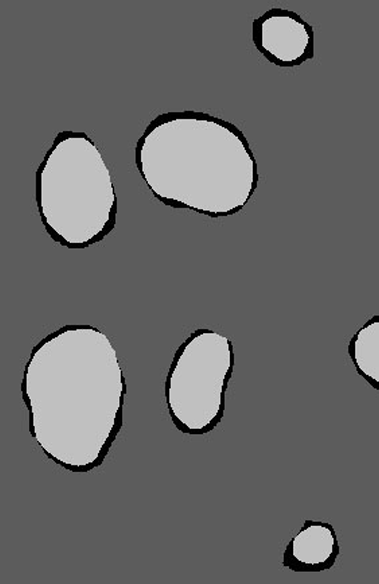
\includegraphics[width=2.5cm]{Definitions/figure-4c.png}}
	\hspace{0.1cm}
	\subfloat[\centering]{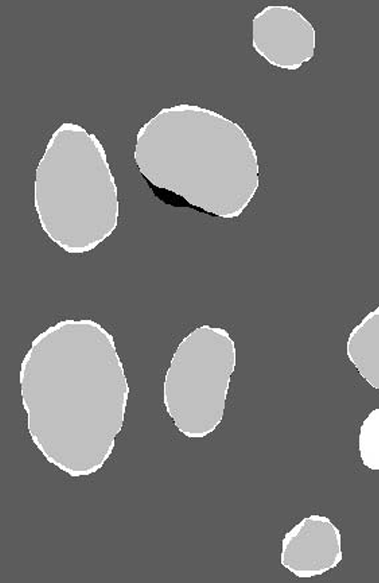
\includegraphics[width=2.5cm]{Definitions/figure-4d.png}}
	\caption{Markup differences (background—dark gray, intersection areas—light gray): (\textbf{a}) original EPFL EM fragment; (\textbf{b}) EPFL (black)/our (white) markup (\textbf{c}) Lucchi++ (black)/EPFL (white) markup (\textbf{d}) Lucchi++ (black)/our (white) markup.\label{fig4}}
\end{figure}

The difference in the results for 42 layers is as follows: Lucchi++ vs. ours, 0.09; EPFL vs. ours, 0.21; Lucchi++ vs. EPFL, 0.19. This is a significant difference. This explains the fact that our test results are better for the Lucci++ markup. At the same time, it can be noted that Lucci++, due to enhanced markup checking compared to EPFL, like our dataset, more correctly solves the problem as a whole.

\subsection{Segmentation Algorithm Stability}

We investigated how stable both are: the process of training the multi-class segmentation of the tiny-U-Net model and the assessment of the segmentation accuracy by this model. It was interesting to obtain such an assessment both on our EPFL6 dataset and on the Lucchi++ dataset to ensure the correctness of using the segmentation assessment as an assessment of the quality of the generated synthetic datasets. It is also important that the dataset we are studying also contains underrepresented classes, which can happen in many cases of technology applications. Therefore, it is also interesting to see how the underrepresentation of a class would look like in such assessments. As a result, the EPFL6 dataset is represented by 42 layers from the training part and 5 layers from the test part (taken for marking from 165 layers of the EPFL test part). The results are presented in Table 2. The Lucchi++ column contains test results for model that trained on 100 (1st line) and 165 (2nd line) layers from the training set and 165 layers from the test set. Note also that the abbreviation “Mit.boundary” stands for “Mitochondrial boundary".

We trained the model 20 times and averaged the results. From Table 2, one can see that the metrics for mitochondria and membranes are quite stable from run to run. The standard deviation is ~0.007 and ~0.002. On the contrary, the results for the axon and PSD vary greatly from run to run.

\begin{table}[H]
	\caption{Stability of segmentation estimation by tiny-U-Net model on EPFL6 and Lucchi++ datase.\label{tab1}}
	\begin{adjustwidth}{-\extralength}{0cm}
		\begin{tabularx}{\fulllength}{CCCCCCCC}
			\toprule
			\textbf{Metric}	& \textbf{Mitochondria}	& \textbf{PSD}	& \textbf{Vesicles}	& \textbf{Axon}	& \textbf{Membrane} & \textbf{Mit.boundary} & \textbf{Lucchi++}\\
			\midrule
				5 classes, Mean & 0.925 & 0.800 & 0.727 & 0.128 & 0.872 & & 0.928\\
				\hline
				5 classes, Std & 0.007 & 0.022 & 0.004 & 0.152 & 0.002 & & 0.006\\
				\hline
				6 classes, Mean & 0.927 & 0.775 & 0.725 & 0.125 & 0.872 & 0.798 & 0.934\\
				\hline
				6 classes, Std & 0.007 & 0.064 & 0.005 & 0.169 & 0.002 & 0.007 & 0.003\\
			\bottomrule
		\end{tabularx}
	\end{adjustwidth}
\end{table}

\subsection{Technology for the Automatic Labeling of Synthetic Classes Based on the Diffusion Mod}

If you take an image and start applying Gaussian noise to it, after a sufficient number of iterations of adding noise, the original image will turn into a pattern of pure noise. The core concept of the diffusion models is to learn how to reverse the described process, gradually removing noise from a noisy image and eventually obtaining a clear image. Based on this, the network architecture should satisfy the following requirement—the input and output should have the same dimensions. An architecture that fulfills these requirements is, for example, the standard U-Net architecture. This approach has been successful in the field of image generation, and models using this method are starting to compete with and even surpass other types of generative models. For instance, such models already outperform Generative Adversarial Networks (GANs) in terms of perceptual quality metrics [28].

The idea of training a model capable of generating both an image and its corresponding annotation is based on creating a training dataset for a diffusion model where each input tensor contains information about the original image and the annotation for that image.

The EPFL dataset was used only as the source data for our own multiclass labeling. The new dataset was generated as follows
\begin{enumerate}
	\item {The data with their annotations, layer-by-layer (in order of layer sequence), are
	combined into one common tensor of size H × W × C, where H and W are the image
	sizes, and C is the number of channels. The C value determines the number of
	channels in the original layer image (in our case, the image is grayscale, that is, one
	channel) plus the number of classes, for each of which a single-channel mask should
	be generated.} 
	\item {The layer image is divided into parts of size 256 × 256 pixels. This is performed
	to avoid scaling the image during the dataset preprocessing before model training,
	which could lead to loss of information about the original image and its details as
	well as blurring of images}
	\item	{For layers, standardization (or Z-Score normalization) is used, and mask normalization (or Min-Max scaling or division by 255) is used. The raw dataset data are
	converted using the following formulas:
	\begin{equation}
		layer_{\text{normalized}} = \frac{layer - mean_{layer}}{std_{layer}}, \quad
    mask_{\text{normalized}} = \frac{mask - min_{mask}}{max_{mask} - min_{mask}} = \frac{mask}{255}
    \tag{4}
	\end{equation}
	}
\end{enumerate}

U-Net from the python library diffusers (https://pypi.org/project/diffusers/, accessed on 2 December 2024) was used as the architecture of the diffusion model. The model was created using a function called UNet2DModel and allows one to obtain a model with additional modifications, such as embedding a position for diffusion time and internal attention blocking.

To create the model, the UNet2DModel function was used from diffusers with the following parameters: $sample\_size$ = 256—sets the width and height of the input data; $in\_channels$ and $out\_channels$ = number of classes + 1 (adding 1 channel for a layer)—set the number of input and output channels; $layers\_per\_block$ = 2—the number of repetitions convolution/deconvolution per block; $block\_out\_channels$ = (128, 128, 256, 256, 512, 512)—list from the number of channels after exiting the blocks (the list has an equal encoder or decoder block); the encoder block contains 4 “DownBlock2D”, after them “AttnDownBlock2D” and “DownBlock2D”; the decoder block contains “UpBlock2D”, “AttnUpBlock2D”, and 4 more blocks “UpBlock2D”.

The resulting model is shaped like U-Net, contains 6 convolutional and deconvolutional layers (or blocks) with skip connections, and also has an attention model (block with Attn) and an input to indicate the current step of the diffusion (or denoising) process.

To return the normalized layers to the previous pixel intensity range of 0–255, the reverse method was applied. For this, the following formula was applied:

\begin{equation}
	image = {image - mean_{\text{after model}}}\ast{std_{layer}}{+}{mean_{\text{train dataset}}}
\end{equation}

where $mean_{\text{train dataset}}$ = 138.84 and $std_{\text{train dataset}}$ = 29.68 are the average and std of the pixel intensities of 42 layers of the EPFL training dataset. This method allows us to avoid shifting the average and std intensity values across channels, which can be observed with other methods of returning the image to the 0–255 range. To return the masks, the pixel values were multiplied by 255.

Figure 5 shows examples of good generation using the diffusion model. Layers of masks are translated into one image, where different classes are marked with different colors: red—the inside area of the mitochondrion, light green—the border of the mitochondrion, green—membranes, blue—vesicles.

\begin{figure}[H]
	\subfloat[\centering]{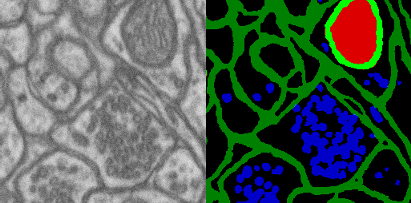
\includegraphics[width=4cm]{Definitions/figure-5a.png}}
	\hspace{0.2cm}
	\subfloat[\centering]{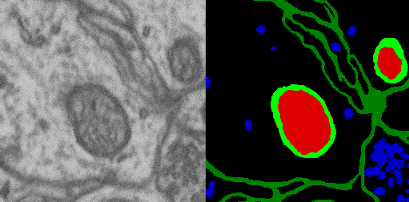
\includegraphics[width=4cm]{Definitions/figure-5b.png}}
	\hspace{0.2cm}
	\subfloat[\centering]{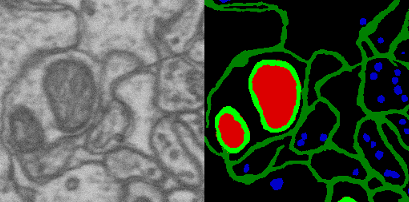
\includegraphics[width=4cm]{Definitions/figure-5c.png}}
	\hspace{0.2cm}
	\caption{Successful examples for the 6-class-labeled synthetic dataset generated by a diffusion model: (\textbf{a-c}) —3 synthetic images and their labeling; the training dataset includes 30 EPFL6 layers.\label{fig5}}
\end{figure}

Examples of unsuccessful generations are also shown (Figure 6) as 3 synthetic images and their labeling masks.

\begin{figure}[H]
	\subfloat[\centering]{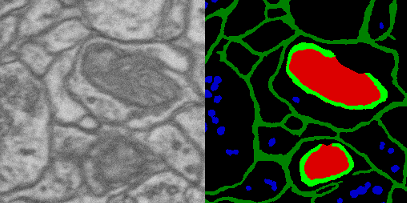
\includegraphics[width=4cm]{Definitions/figure-6a.png}}
	\hspace{0.2cm}
	\subfloat[\centering]{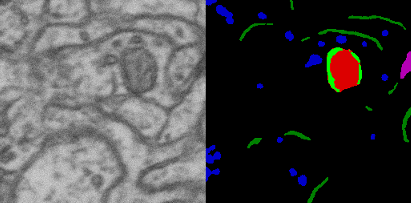
\includegraphics[width=4cm]{Definitions/figure-6b.png}}
	\hspace{0.2cm}
	\subfloat[\centering]{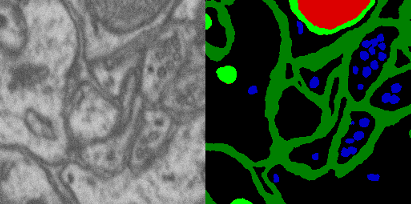
\includegraphics[width=4cm]{Definitions/figure-6c.png}}
	\hspace{0.2cm}
	\caption{Examples of mistakes for the 6-class-labeled synthetic dataset generation via a diffusion
	model. The mask shows mitochondria boundaries having gaps: (\textbf{a,b}) the membrane mask does not quite match the layer; (\textbf{c}) mitochondria consisting of only the boundary class.\label{fig6}}
\end{figure}

Examples of axon generations are shown in (Figure 7).

\begin{figure}[H]
	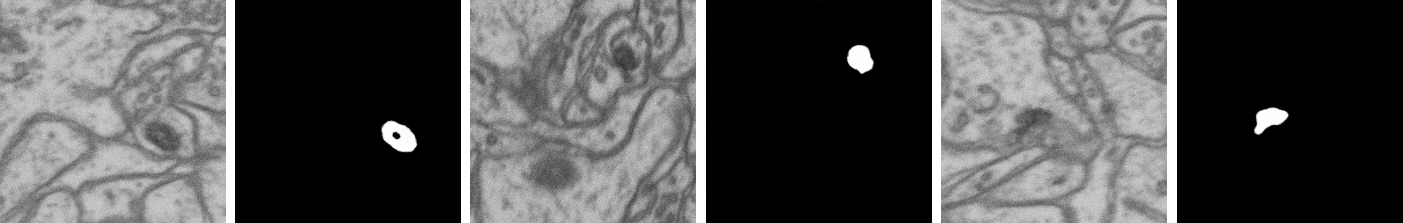
\includegraphics[width=13cm]{Definitions/figure-7.png}
	\caption{Example of synthesized data by DIFF 6-class (42-layer) diffusion model. Synthetic tile
	(fragment) and it’s axon masks.}
\end{figure}

\subsection{Geometric Models for Dataset Synthesis}

The research presented in this section is a development of our work [34 ,35 ]. We present new samples of synthetic images generation as the main method of augmentation for classes that are underrepresented in the dataset. In the EPFL dataset, this is an axon class (see Figure 3).

The essence of the geometric algorithm is that organelles are drawn using simple geometric primitives such as lines, splines, and area fills. The sizes and gray levels for organelles are set based on data from the target dataset. A complex internal structure is also applied by adding lines, circles, spline pieces, and blurs to the selected area. Membranes are calculated using a region-growing algorithm. We used Gauss filtering and Poisson noise to simulate image blurring and noise from the registration device. Drawing masks repeats the algorithm for drawing organelles, only without blurring and adding noise. One can see and download the implementation of our algorithms for geometric synthesis here: \href{https://github.com/GraphLabEMproj/Synthetics/}{https://github.com/GraphLabEMproj/Synthetics/}, accessed on 2 December 2024. A description of the geometric synthesis algorithms can be found in [35].

This is why, for the geometric synthesized dataset, we generated 2000 images of size 256 × 256 pixels; half of this dataset contained the axon area. An example of one labeled sample and an example of several samples are shown in Figure 8. The shape, size, and gray levels of compartments are chosen to be similar to the shape, size, and gray levels of the EPFL dataset. The advantage of a synthetic set is that you can obtain any number of images you need along with their labeling automatically.

\begin{figure}[H]
	\subfloat[\centering]{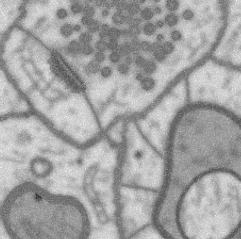
\includegraphics[width=2cm]{Definitions/figure-8a.png}}
	\hspace{0.1cm}
	\subfloat[\centering]{
\includegraphics[width=2cm]{Definitions/figure-8b.png}}
	\hspace{0.1cm}
	\subfloat[\centering]{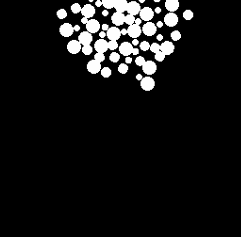
\includegraphics[width=2cm]{Definitions/figure-8c.png}}
	\hspace{0.1cm}
	\subfloat[\centering]{
\includegraphics[width=2cm]{Definitions/figure-8d.png}}

	\vspace{0.1cm}

	\subfloat[\centering]{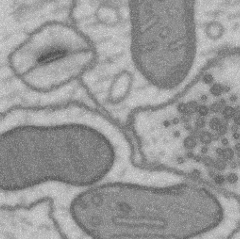
\includegraphics[width=2cm]{Definitions/figure-8e.png}}
	\hspace{0.1cm}
	\subfloat[\centering]{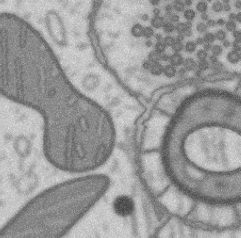
\includegraphics[width=2cm]{Definitions/figure-8f.png}}
	\hspace{0.1cm}
	\subfloat[\centering]{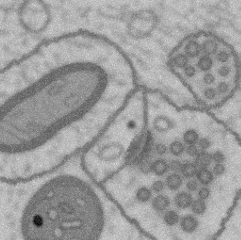
\includegraphics[width=2cm]{Definitions/figure-8g.png}}
	\hspace{0.1cm}
	\subfloat[\centering]{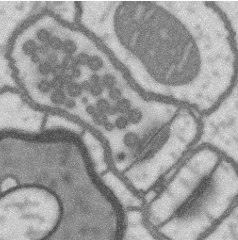
\includegraphics[width=2cm]{Definitions/figure-8h.png}}
	\caption{Example of geometric synthesized data: (\textbf{a}) layer; (\textbf{b}) mask of axons’ sheaths; (\textbf{c}) mask of vesicles; (\textbf{d}) PSD mask; (\textbf{e-h}) examples of synthetic layers.\label{fig8}}
\end{figure}

\subsection{Naturalization of Geometric and Other Synthetic Datasets by Diffusion Models}

The Table 3 shows that geometric synthetics have a significant drawback due to their schematic and complexity of the brain cell shapes. The column best results are highlighted by the bold font, and the best for left or right halftable by the gray background.

Diffusion networks do a great job of synthesizing textured objects such as mitochondria and clusters of vesicles, but diffusion neural networks cannot confidently model properties that geometric synthetics can guarantee: membrane continuity and PSD placing. We decided to combine the strengths of diffusion and geometric synthetics by naturalizing the result of geometric synthetics with a diffusion model. To do this, an experiment was conducted to determine both the possibility of such a naturalization method and adequate proportions for mixing the models. In this experiment, images of geometric synthetics were noisy to a level determined by the coefficient $\alpha$ and then fed for denoising to the input of a diffusion model trained on the original data. For a number of values of $\alpha$, the naturalization of the geometric model reaches a level equal to the result of applying the diffusion model to the original dataset.

We used a geometric synthetic image as the initial image and made it noisy as required by the diffusion model. The noisy image is fed to the input of the diffusion model in Section 2.4 and trained on images of the original dataset. The input of the model forms one common tensor from the layers of the original layer and the mask; this entire tensor is noisy and restored by diffusion. For masks, the operations are the same as for a layer. Therefore, if diffusion corrects the layer, it also corrects the masks. We tested 20 levels of added noise (see Figure 9).

\begin{table}[H]
	\caption{Dice coefficient of electron microscopy data segmentation for the tiny-U-Net model for the original EPFL6 dataset (ORIG), the dataset enriched with diffusion-synthesized images (MIX), and the fully diffusion-synthesized dataset (DIFF)}
		\begin{adjustwidth}{-\extralength}{0cm}
			{\fontsize{9.35pt}{10pt}\selectfont
			\begin{tabularx}{\fulllength}{ccccccc|cccccc}
				\toprule
					\multirow{3}{*}{\textbf{Num}} & \multicolumn{12}{c}{\textbf{Training Dataset}}\\
				\cmidrule(lr){2-13}
					& \multicolumn{2}{c}{\textbf{MIX}} & \multicolumn{2}{c}{\textbf{DIFFUSION}} & \multicolumn{2}{c|}{\textbf{ORIGINAL}} & \multicolumn{2}{c}{\textbf{MIX}} & \multicolumn{2}{c}{\textbf{DIFFUSION}} & \multicolumn{2}{c}{\textbf{ORIGINAL}}\\
      		& \textbf{MIX 5} & \textbf{MIX 6} & \textbf{DIFF 5} & \textbf{DIFF 6} & \textbf{ORIG 5} & \textbf{ORIG 6} & \textbf{MIX 5} & \textbf{MIX 6} & \textbf{DIFF 5} & \textbf{DIFF 6} & \textbf{ORIG 5} & \textbf{ORIG 6}\\
      	\midrule
					& \multicolumn{6}{c}{\textbf{Mitochondria}} & \multicolumn{6}{c}{\textbf{Mitochondria Boundaries}}\\
				\cmidrule(lr){1-13}
					5 & 0.860 & 0.886 & 0.850 & 0.871 & 0.882 & 0.885 & 0.880 & 0.760 & 0.835 & 0.741 & 0.877 & 0.752\\
					10 & 0.943 & 0.935 & \textbf{0.936} & 0.906 & \textbf{0.934} & 0.928 & 0.921 & 0.797 & 0.910 & 0.752 & 0.916 & 0.787 \\
					15 & \textbf{0.945} & \textbf{0.942} & 0.930 & 0.937 & 0.930 & 0.926 & 0.918 & 0.793 & 0.876 & \textbf{0.762} & \textbf{0.914} & 0.790\\
					20 & 0.939 & 0.938 & 0.931 & \textbf{0.941} & 0.924 & 0.925 & \textbf{0.925} & 0.795 & \textbf{0.924} & 0.754 & 0.912 & 0.794\\
					30 & 0.932 & \textbf{0.942} & 0.895 & 0.928 & 0.922 & 0.924 & 0.924 & \textbf{0.799} & 0.916 & 0.751 & 0.913 & \textbf{0.796}\\
				\midrule
					& \multicolumn{6}{c}{\textbf{PSD}} & \multicolumn{6}{c}{\textbf{Membranes}}\\
				\cmidrule(lr){1-13}
					5 & 0.672 & 0.654 & 0.513 & 0.582 & 0.556 & 0.566 & 0.868 & 0.868 & 0.849 & \textbf{0.852} & 0.861 & 0.862\\
					10 & 0.820 & 0.783 & 0.735 & 0.532 & 0.755 & 0.754 & 0.869 & \textbf{0.872} & \textbf{0.854} & 0.847 & \textbf{0.872} & \textbf{0.873}\\
					15 & 0.723 & 0.755 & 0.621 & 0.643 & 0.685 & 0.697 & 0.869 & 0.864 & 0.844 & 0.814 & 0.871 & 0.872\\
					20 & \textbf{0.821} & 0.773 & \textbf{0.748} & 0.731 & 0.755 & 0.726 & 0.865 & 0.864 & 0.831 & 0.813 & 0.871 & \textbf{0.873}\\
					30 & 0.816 & \textbf{0.810} & 0.472 & \textbf{0.783} & 0.723 & 0.766 & 0.872 & 0.864 & 0.849 & 0.791 & \textbf{0.872} & \textbf{0.873}\\
				\midrule
					& \multicolumn{6}{c}{\textbf{Vesicles}} & \multicolumn{6}{c}{\textbf{Axon}}\\
				\cmidrule(lr){1-13}
					5 & 0.692 & 0.697 & 0.687 & 0.693 & 0.689 & 0.686 & 0.020 & 0.043 & 0.023 & 0.036 & 0.144 & 0.282\\
					10 & \textbf{0.734} & 0.719 & 0.727 & 0.724 & 0.718 & 0.720 & 0.009 & 0.062 & 0.013 & \textbf{0.178} & \textbf{0.304} & 0.265\\
					15 & 0.730 & 0.728 & 0.735 & 0.725 & 0.716 & 0.724 & 0.012 & 0.043 & 0.013 & 0.024 & 0.122 & 0.274\\
					20 & \textbf{0.734} & 0.728 & \textbf{0.736} & 0.729 & 0.714 & 0.717 & 0.010 & 0.022 & 0.097 & 0.243 & 0.181\\
					30 & 0.725 & \textbf{0.735} & 0.731 & 0.730 & 0.722 & 0.724 & 0.010 & 0.376 & 0.007 & 0.192 & \textbf{0.312}\\
				\bottomrule
			\end{tabularx}
			}
		\end{adjustwidth}
\end{table}

\section{Results}

The experiment was designed as a two-stage one: Stage 1—synthesis of a multi-class dataset by a diffusion model trained on EPFL6; Stage 2—evaluation on the test part of EPFL6 of the accuracy of multi-class segmentation trained on its training part. Before discussing the obtained results and to understand them better, it is worth clarifying how the training datasets for the diffusion model and for the segmentation model were formed in each experiment, on whose test dataset the segmentation accuracy was checked.

First of all, we note that only two original datasets were used in the experiments: EPFL, marked up for one class of mitochondria, in the refined Lucchi++ markup; EPFL6 with our markups for one, five, and six classes. Only one designation is used for EPFL6. EPFL with the refined markup of mitochondria is designated as Lucchi++ or Lucchi for short in the tables and explanatory texts. Lucchi++ has two parts, training and testing, with 165 layers each. From EPFL6, from 5 to 42 layers from the training part and 5 layers from the testing part were used in the experiment. For the augmentation of 5 EPFL6 test layers, regular tiling with a 256 × 256 window with an offset of 128 was used, giving 35 [tiles/layer] instead of 12 [tiles/layer] (without overlapping). Regardless of how many layers are used to train the model, all test layers of the corresponding datasets are used for testing. All tables show Dice values averaged over several (from 5 to 20) implementations.

The size of the synthetic datasets is practically unlimited, but for resource conservation reasons, 1008 disjoint images of size 256 × 256 were generated for any size of the training dataset, equivalent to 84 standard EPFL 1024 × 768 layers, i.e., 12 images per layer. Synthetic datasets were generated once, a separate dataset was generated for each combination of the number of classes and number of training layers. Their naming is more diverse and is tied to the result tables. To increase the volume of the training dataset, regular tiling was applied to its layers with a tile size of 256 × 256 and an offset of 64 (or 128), selected based on the experiment. The number of tiles in a layer when tiling without tile intersections is 12 (4 × 3). With an offset of 128, the number of tiles k is determined by the formula k = (2n - 1) x (2m - 1), where n = 4, m = 3, and k = 35 = 7 x 5. The next division of the offset by 2 gives, according to the same formula, k = 117 = (2 × 7– 1)(2 × 5– 1). That is, when training on L layers, we have the following pairs in the training dataset: [number of layers, number of intersecting 256 × 256 tiles]: [5, 585], [10, 1170], [15, 1755], [20, 2340], [30, 3510], [42, 4914]. In this case, the number of diffusion synthetic images generated on each training dataset, as indicated above, remained constant in all experiments and was equal to 1008 tiles. This option is interesting because it allows us to compare the segmentation accuracy when training on an increasing and constant dataset volume. The only exception is made for the five-layer dataset, in which the DIFF synthetic training dataset is represented by 595 out of 1008 images.

For the computational experiment, the nodes of the supercomputer (SC) Lobachevsky (LobachevskyUniversity, NizhnyNovgorod) (\href{https://hpc-education.unn.ru/en/resources}{https://hpc-education.unn.ru/en/resources}, accessed on 2 December 2024), equipped with eight graphic processors (GPUs) A100, 40 GB, were used. A total of 100 epochs were allocated for the training process of the diffusion model on the original datasets formed from the EPFL6 composition, which took about 2.5 h A100, 40 GB. The process of generating a synthetic dataset of 1008 images of size 256 × 256 for each of the markings (1, 5, 6 classes) by the trained model took about 5 h GPU A100, 40 GB. The time on the computing node together with loading and unloading was about 8 hfor one synthetic dataset of 1008 images of the above size. A total of 200 epochs were allocated for the training process of the tiny-U-Net segmentation model.

\subsection{Software and Technologies for Training and Testing}

We used Python as the main programming language to conduct experiments. The main libraries for working with deep learning are PyTorch and Diffusers. PyTorch is chosen as one of the most popular libraries for DL. The Diffusers library, based on PyTorch, contains functions for creating and training models using diffusion technology.

Training deep learning models requires a large amount of data to reduce the possibility of overfitting. At the same time, the larger the model, the more data it requires. To increase the amount of data for training, we sliced the training layers into tiles of 256 × 256 pixels. In our previous works, we used 256 × 256 slicing with an offset of 128 and 512 × 512 with an offset of 256, which allowed us to obtain 41 tiles per layer. Thus, for 42 layers, 1722 tiles of training data were obtained. When conducting initial experiments with the standard diffusion model, which is large in size, the generation results after training were unsatisfactory, so it was decided to increase the training dataset by reducing the slicing bias to 64. Therefore, in this work, slicing the layer into 256 × 256 tiles with an offset of 64 was used to train the models. This allowed for obtaining 117 tiles from a single 1024 × 768 pixel layer. It is worth noting that these data are not diverse due to multiple overlaps. From one 1024 × 768 layer, only 12 tiles of a size of 256 × 256 can be obtained without intersections, so expanding the dataset by slicing with an offset increases its diversity nonlinearly and loses its power at small values.

U-Net, despite its architecture, may still face difficulties when processing image edges. To avoid artifacts at the edges of tiles, we cut the test image into overlapping tiles.

We prepared tiles with a size of 256 × 256 pixels and an overlap of 128 pixels for testing. Only the centers of the 128 × 128 pixel regions within these tiles are included in the final mask (see Figure 9)

\begin{figure}[H]
	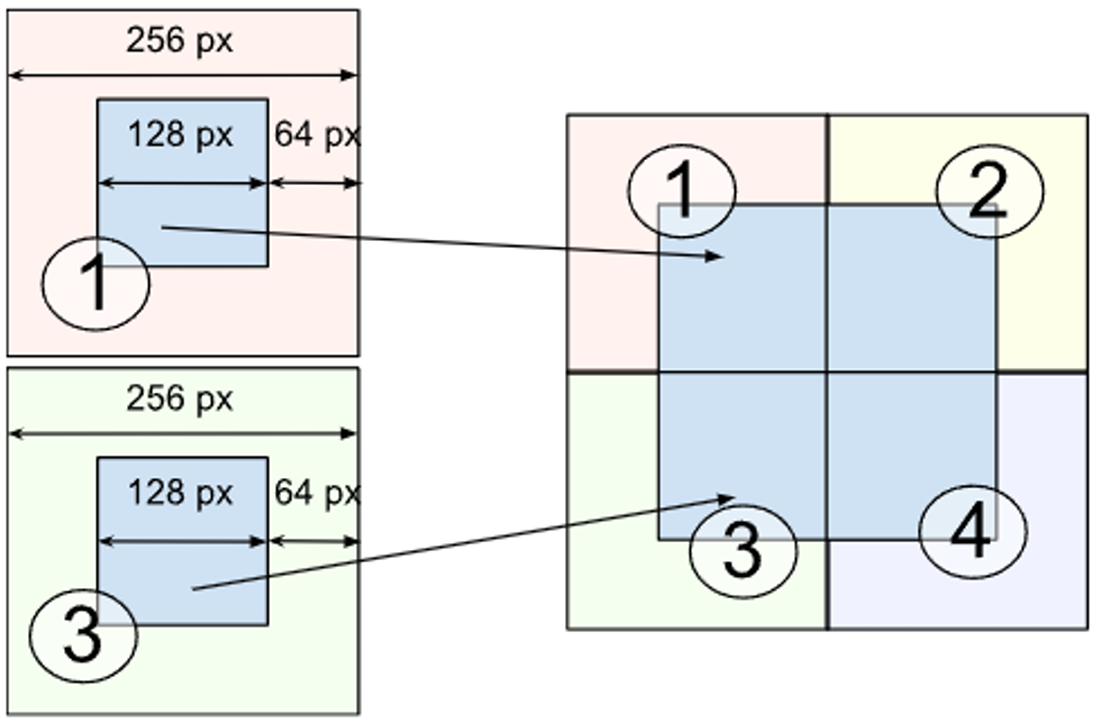
\includegraphics[width=8 cm]{Definitions/figure-9.png}
	\caption{Process of splitting a test image into.\label{fig9}}
\end{figure}

\subsection{Generation of Synthetic Multi-class Datasets by Diffusion Model}

The U-Net model was trained with the following hyperparameters: input and output image sizes = 256 × 256 × (N + 1) pixels, where N is the number of classes; batch size for training set = 12; number of training epochs = 100; learning rate for optimizer = 0.0004; number of denoising steps = 700.

With these parameters, we generated the next 1000-tiles training volumes:

\begin{itemize}
	\item {DIFF 6-class 42 layers: 42 layers from the EPFL6 training dataset, all six classes (the example: see Figure 10). The diffusion model was trained on this dataset, and this model synthesized the input datasets DIFF 6 and MIX 6 (with the addition of the EPFL6 dataset images) for the segmentation task in Tables 3 and 4.}
	\item {DIFF 5-class 42 layers: 42 layers from the EPFL6 training dataset, five classes of markup. The diffusion model was trained on this dataset, and this model synthesized the input datasets DIFF 5 and MIX 5 (with the addition of images from the EPFL6 dataset) for the segmentation task in Tables 3 and 4.}
	\item {DIFF 1-class 42 layers: 42 layers from the EPFL6 training dataset, one class of markup. The diffusion model was trained on this dataset, and this model synthesized the input datasets DIFF 1 and MIX 1 (as a fusion with the images from the EPFL6 dataset) for the segmentation task in Table 4}
	\item {DIFF 1-class 165 layers: 165 images from the EPFL one-class training dataset in Lucchi++ labeling. The diffusion model trained on this dataset synthesized the input dataset for the combination: Lucchi++ plus DIFF 1(165), 84 (Table 5)}
\end{itemize}

\begin{figure}[H]
	\subfloat[\centering]{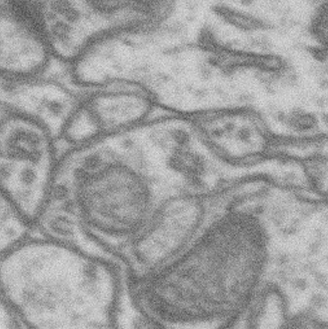
\includegraphics[width=2.5cm]{Definitions/figure-10a.png}}
	\hspace{0.1cm}
	\subfloat[\centering]{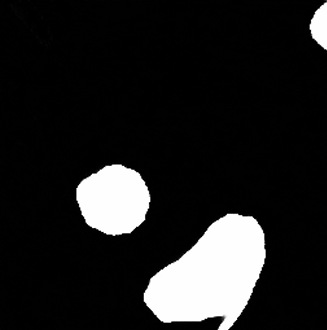
\includegraphics[width=2.5cm]{Definitions/figure-10b.png}}
	\hspace{0.1cm}
	\subfloat[\centering]{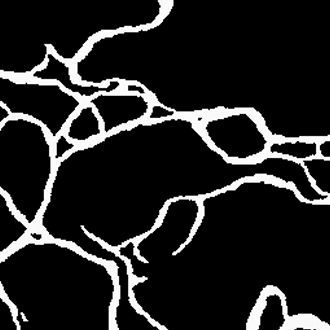
\includegraphics[width=2.5cm]{Definitions/figure-10c.png}}
	\hspace{0.1cm}
	\subfloat[\centering]{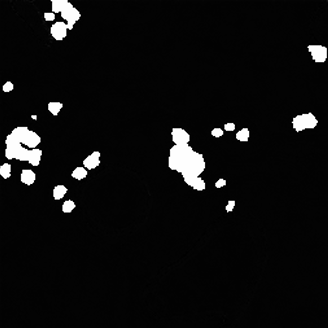
\includegraphics[width=2.5cm]{Definitions/figure-10d.png}}
	\hspace{0.1cm}
	\subfloat[\centering]{
\includegraphics[width=2.5cm]{Definitions/figure-10e.png}}
	\hspace{0.1cm}
	\caption{Example of synthesized dataset DIFF 6-class 42 layers (only nonzero masks are shown): (\textbf{a}) the synthetic layer; (\textbf{b}) mitochondria mask; (\textbf{c}) membranes mask; (\textbf{d}) vesicles mask; (\textbf{e}) PSD mask.\label{fig10}}
\end{figure}

\begin{table}[H] 
	\caption{Dice coefficient for EPFL6-based synthetic data segmentation by tiny-U-Net model. The table has 3 main sections: Original datasets; Synthetic datasets; Mixed two firsts, - for 3 types of synthetic.}
	\begin{adjustwidth}{-\extralength}{0cm}
		{\fontsize{10pt}{10pt}\selectfont
		\begin{tabularx}{\fulllength}{CCCCCCC}
			\toprule
			\textbf{Metric} & \textbf{Mitochondria}	& \textbf{PSD}	& \textbf{Vesicles}	& \textbf{Axon}	& \textbf{Membranes}	& \textbf{Mit. Boundaries}\\
			\midrule
			MIX NAT 1 & 0.920 & - & - & - & - & -\\
			MIX NAT 5 & 0.924 & \textbf{0.851} & 0.708 & 0.527 & 0.876 & -\\
			MIX NAT 6 & 0.928 & 0.842 & 0.716 & 0.534 & \textbf{0.877} & 0.802\\
			MIX DIFF 1 & 0.927 & - & - & - & - & -\\
			MIX DIFF 5 & \textbf{0.944} & 0.833 & \textbf{0.734} & 0.017 & 0.867 & -\\
			MIX DIFF 6 & 0.939 & 0.841 & 0.732 & 0.000 & 0.869 & 0.805\\
			MIX GEOM 1 & 0.926 & - & - & - & - & -\\
			MIX GEOM 5 & 0.936 & 0.836 & 0.725 & \textbf{0.789} & 0.871 & -\\
			MIX GEOM 6 & 0.933 & 0.845 & 0.721 & 0.722 & 0.873 & \textbf{0.807}\\
			\midrule
			SYN NAT 1 & 0.883 & - & - & - & - & -\\
			SYN NAT 5 & 0.885 & 0.701 & 0.510 & 0.565 & 0.810 & -\\
			SYN NAT 6 & 0.839 & 0.652 & 0.512 & 0.542 & 0.793 & 0.638\\
			SYN DIFF 1 & 0.918 & - & - & - & - & -\\
			SYN DIFF 5 & \textbf{0.942} & 0.781 & \textbf{0.736} & 0.072 & \textbf{0.839} & -\\
			SYN DIFF 6 & \textbf{0.942} & \textbf{0.808} & 0.730 & 0.025 & 0.831 & \textbf{0.775}\\
			SYN GEOM 1 & 0.891 & - & - & - & - & -\\
			SYN GEOM 5 & 0.905 & 0.704 & 0.623 & 0.882 & 0.792 & -\\
			SYN GEOM 6 & 0.905 & 0.708 & 0.609 & \textbf{0.898} & 0.790 & 0.704\\
			\midrule
			ORIGINAL 1 & 0.913 & - & - & - & - & -\\
			ORIGINAL 5 & \textbf{0.928} & \textbf{0.824} & \textbf{0.732} & \textbf{0.133} & 0.872 & -\\
			ORIGINAL 6 & \textbf{0.928} & 0.814 & 0.724 & 0.070 & \textbf{0.873} & 0.799\\
			\bottomrule
		\end{tabularx}
		}
	\end{adjustwidth}
\end{table}

We constructed histograms to visualize the statistics of the datasets, as presented in Figure 11. The histograms of real and synthetic datasets are indeed very similar, but the range of values in the real image is slightly wider. Based on the histogram comparison, it can be concluded that the diffusion model predominantly generates images similar to the original dataset. By visual analysis it was found that a small part of the generation contains errors. Examples of successful and unsuccessful generations are shown in Figures 5 and 6. However, this part containing errors was not excluded from the d

\begin{table}[H] 
	\caption{Comparison with existing mitochondrial segmentation methods.}
		\begin{tabularx}{\textwidth}{CCC}
			\toprule
			\textbf{Methods}	& \textbf{Labeling}	& \textbf{Dice}\\
			\midrule
				HIVE-net [43] & Lucchi++ & 0.948\\
				tiny-U-Net \textsuperscript{2} & Lucchi++ plus DIFF 1 (165), 84 & 0.946\\
				tiny-U-Net \textsuperscript{2} & Lucchi++ & 0.934\\
				tiny-U-Net \textsuperscript{2} & Lucchi++, 100 (out of 165) & 0.928\\
				tiny-U-Net \textsuperscript{2} & DIFF 1 (165), 84 & 0.927\\
				tiny-U-Net \textsuperscript{2} & DIFF 6 (42), 84 & 0.917\\
				tiny-U-Net \textsuperscript{2} & Lucchi++, 42 (out of 165) & 0.913\\
				3D Casser et al. [41] \textsuperscript{1} & Lucchi++ & 0.942\\
				Cheng et al. (3D) [44] \textsuperscript{1} & Lucchi++ & 0.941\\
				3D U-Net [11] \textsuperscript{1} & Lucchi++ & 0.935\\
				Cheng et al. (2D) [44] \textsuperscript{1} & Lucchi++ & 0.928\\
				U-Net [7] \textsuperscript{1} & Lucchi++ & 0.915\\
				Peng et al. [45] \textsuperscript{1} & Lucchi++ & 0.909\\
				3D Xiao et al. [10] \textsuperscript{1} & Lucchi++ & 0.900\\
				Cetina et al. [46] \textsuperscript{1} & Lucchi++ & 0.864\\
				Lucchi et al. [5] \textsuperscript{1} & Lucchi++ & 0.860\\
			\bottomrule
		\end{tabularx}
	\noindent{\footnotesize{\textsuperscript{1} The Dice coefficient was taken from article [43]. \textsuperscript{2} This article.}}
\end{table}

\begin{figure}[H]
	\subfloat[\centering]{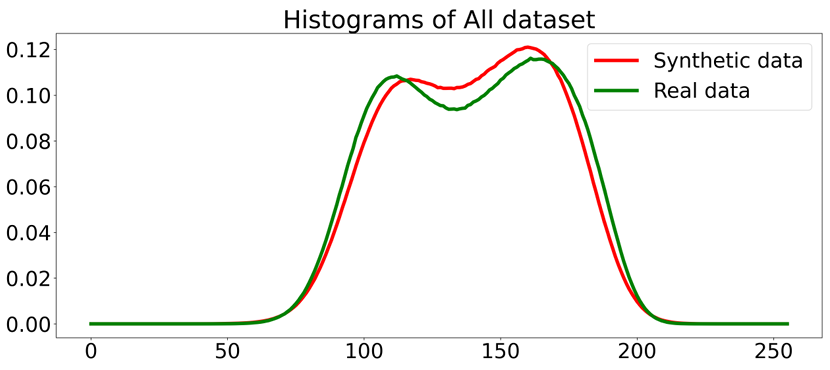
\includegraphics[width=6.5cm]{Definitions/figure-11a.png}}
	\hspace{0.2cm}
	\subfloat[\centering]{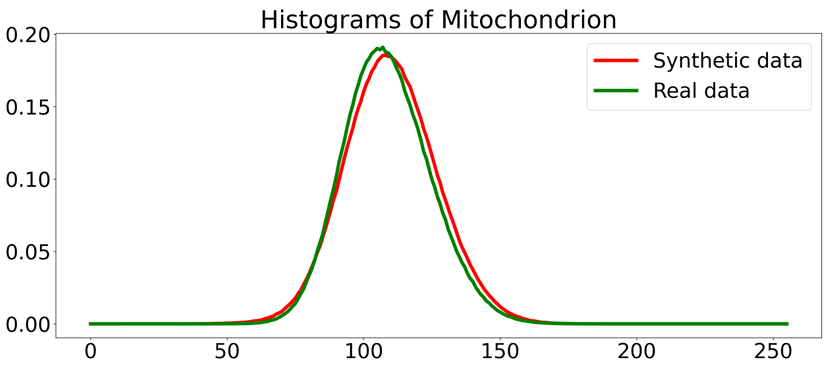
\includegraphics[width=6.5cm]{Definitions/figure-11b.png}}
	\caption{Histograms of the dataset DIFF 6-class 42 layers (histogram of the original dataset in green, histogram of the synthetic dataset in red): (\textbf{a}) histograms of all dataset; (\textbf{b}) histograms of mitochondrion.\label{fig11}}
\end{figure}

\subsubsection{Training a Segmentation Neural Network on a Dataset Using Synthetic Images Generated by a Diffusion Model}

In our previous work [35 ], we used a simplified U-Net model for segmentation (named tiny-U-Net). For mitochondria segmentation, tiny-U-Net demonstrated very close assessments like classical U-Net. The lightweight model contains 15.7 times fewer parameters and occupies 24 MB of RAM instead of 364 MB when using the original model.

The model was trained with the following hyperparameters:

\begin{itemize}
	\item {Input and output image size: 256 × 256 pixels;}
	\item {Batch size for the training set: 7;}
	\item {Number of epochs: 20}
	\item {Adam optimizer with a variable learning rate from 1 x 10\textsuperscript{-4} to 1 x 10\textsuperscript{-6}.}
\end{itemize}

The results of the multi-class segmentation of the electron microscopy data for the tiny-U-Net model for the EPFL dataset and the diffusion dataset are presented in Table 3. The numbers 5 and 6 indicate how many classes the diffusion model was trained for and how many classes the segmentation model was trained for. Our training dataset is EPFL6 with (5, 10, 15, 20, 30) layers. The test dataset is EPFL6. The best value of the two is in italics, the best value in the line is in bold, and the best value in the class is marked in light gray.

\subsubsection{Experiments on Geometric Model for Dataset Synthesis}

In order to determine the effectiveness of using the geometric expansion of the dataset, we trained the neural network on datasets:

GEOM is a training dataset that includes only geometric synthetic data. To obtain a geometric synthetic (GEOM) training dataset, we generated 2000 synthesized fragments of size 256 × 256.

MIX (GEOM) is a mixed training dataset. It includes 4914 fragments of EPFL6 (42 layers of the EPFL6 training dataset cut into 256 × 256 fragments, with an offset of 64 pixels) data and 2000 geometric synthesized fragments; thus, we have 6914 fragments in total.

To additionally increase the training datasets, we made random rotations of images, random shifts, and random scale changes in a small range (50\%) . We selected 20\% of images from the training sample into a validation sample. The batch size was equal to seven.

We used Adam’s optimizer with a dynamic learning rate from 1 × 10\textsuperscript{-4} to 1 × 10\textsuperscript{-6}. The learning rate after the 100th epoch decreased by 5 times, and this was repeated every 25 epochs.

We trained models for one, five, and six classes. The number of epochs in all experiments was 200. The Dice coefficients are presented in Table 4. The mitochondrial boundaries class is a subclass of the class of mitochondria with their boundaries, and the additional edge enhancement improves the segmentation results of the unifying class.

In commercial applications based on deep learning, in addition to quality metrics, the performance characteristics of algorithms also play a large role. Based on the values of the Dice quality metric given in Table 4 (the results for U-Net can be found in [ 34 ]), we see that with a tenfold decrease in the number of model weights (and, hence, the execution time), the results of the quality of work remain comparable.

\subsubsection{Naturalization Results}

Based on the testing results, it can be said that the diffusion model improves the texture of the inner region of the mitochondria well and improves the appearance of the PSD and vesicles. However, this improvement does not cope with those classes that are poorly represented in the training dataset. For example, in the original training dataset, the axon is represented by a single instance of a small size. Following this, the trained diffusion model tries to reduce by several times the area-size of the axon generated by the geometric model. For example, $\alpha$ = 4/20 or $\alpha$ = 11/20 and 14/20 and 14/20.

We can see the results in the NAT columns of Table 4 (augmentation due to the fusion of geometric and diffusion synthetics).

\subsection{Results’ Comparison}

Table 4 presents the results of a comparative experiment of segmentation models for different types of synthetics. The ORIGINAL-prefixed rows indicate 42 layers of the EPFL6 train dataset. The rows entitled MIX indicate a mixed dataset: 42 original layers + synthetics. The type of synthetics is specified by the second word: GEOM—geometric synthetics; DIFF—diffusion synthetics, NAT—naturalization of geometric synthetics by diffusion model with $\alpha$ = 0.5. The best value of the type MIX, SYN, or ORIGINAL is in bold font, and the best value in the class is marked in a light gray background. Test dataset of EPFL6 has five test layers.

In this section, we also visualize segmentation masks to provide a clearer understanding of the comparative results previously analyzed. By overlaying the masks on the original images, we highlight the differences between the ground truth and model predictions: the ground truth boundaries are shown in green, while the predicted boundaries are displayed in red. For visualization, we choose three models corresponding to the MIX NAT 5, MIX DIFF 5, and MIX GEOM 5 rows in Table 4.

Figure 12 shows that the MIX GEOM 5 model copes with axon segmentation significantly better than the others. The model MIX NAT 5 highlights the axon boundaries, while MIX DIFF 5 highlights almost nothing.

\begin{figure}[H]
	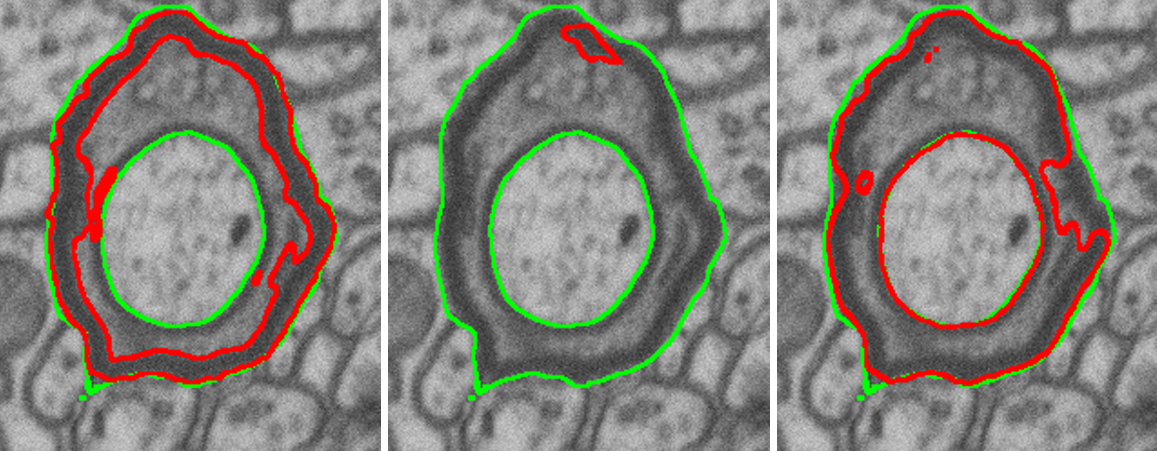
\includegraphics[width=13.5 cm]{Definitions/figure-12.png}
	\caption{Axon prediction from left to right: MIX NAT 5 model prediction, MIX DIFF 5 model prediction, MIX GEOM 5 prediction.\label{fig12}}
\end{figure}

The segmentation results for the vesicles and mitochondria classes are comparable, as evidenced by their similar Dice scores in Table 4. However, the diffusion model demonstrates superior performance in accurately identifying the boundaries of vesicles, highlighting its ability to capture finer details in these structures (see Figures 13 and 14).

\begin{figure}[H]
	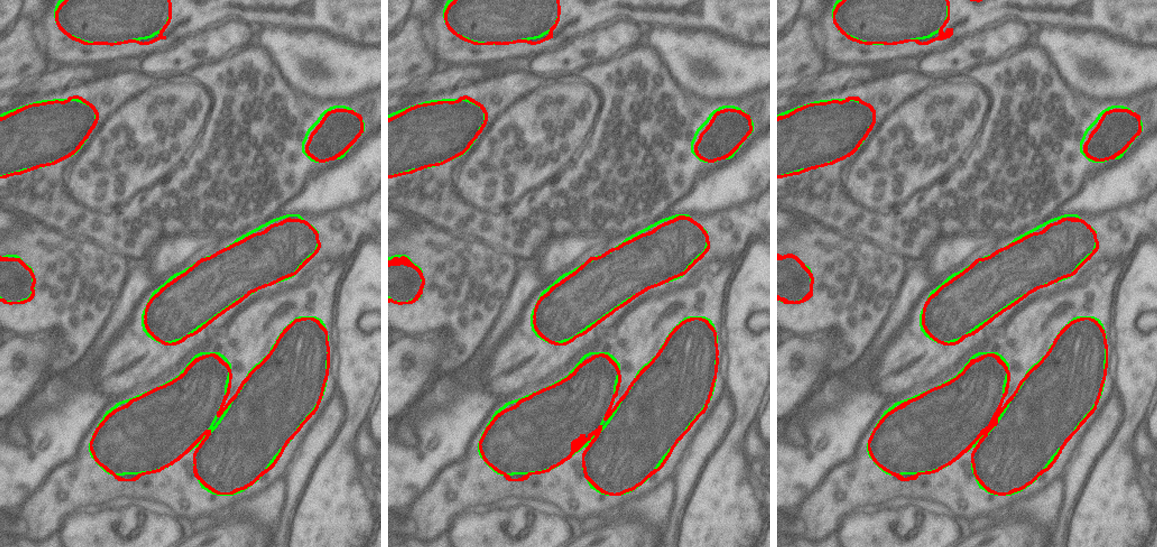
\includegraphics[width=13.5 cm]{Definitions/figure-13.png}
	\caption{Mitochondria prediction from left to right: MIX NAT 5 model prediction, MIX DIFF 5 model prediction, MIX GEOM 5 prediction.\label{fig13}}
\end{figure}

\begin{figure}[H]
	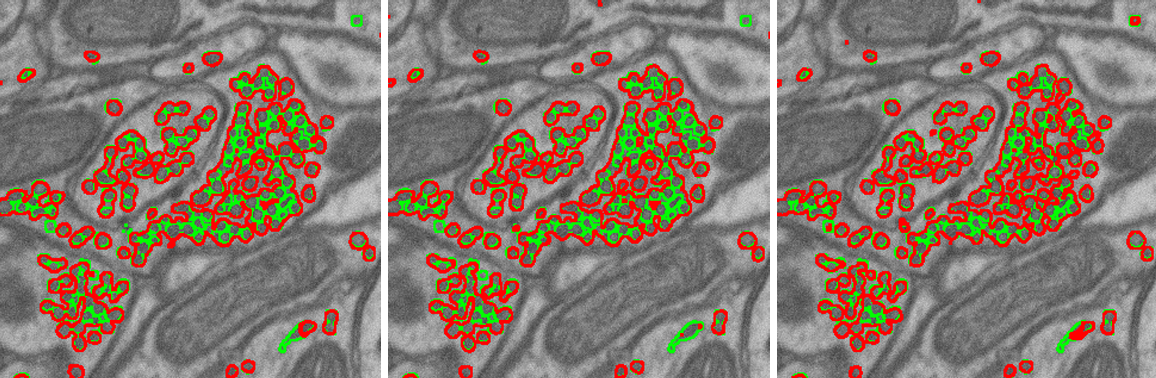
\includegraphics[width=13.5 cm]{Definitions/figure-14.png}
	\caption{Vesicle prediction from left to right: MIX NAT 5 model prediction, MIX DIFF 5 model prediction, MIX GEOM 5 prediction.\label{fig14}}
\end{figure}

\section{Discussion}

Table 3 contains the results of segmentation quality when training on synthetic datasets
generated by the diffusion model. For testing, we used a comparison of class segmentation
accuracies by the tiny-U-Net model trained on (1) the original EPFL6 dataset (ORIGn),
(2) diffusion synthetic datasets (DIFFn), (3) original dataset augmented by the synthetic
one (MIXn).

The results are shown for all classification objects and for all three labels: for one class (mitochondria), five and six classes. The data are averaged over five training runs of the segmentation neural network. The accuracy dependence on the training dataset size is analyzed for a small number of layers compared to Lucchi++. The results for mitochondria are given in the upper data strip: for five and six classes in the left half of the strip, the single-class labeling is moved, for the sake of table compactness, to the left columns of the right half of the strip, and the results for the sixth class of mitochondrial boundary are in the right columns. The dependencies on the number of layers in the training dataset behave similarly. When moving from 5 layers to 10 layers, a noticeable increase in accuracy is visible. Further, on the original data for all three markups, the accuracy remains almost constant, but the accuracy of mitochondria segmentation for classes 5 and 6 is noticeably higher than for the single-class markup. On the diffusion dataset, the average, by the number of layers, accuracy of the single-class markup is slightly worse than for ORIG 1. For classes 5 and 6, the average, by the number of layers, values are close to ORIG 1, but the maximums are noticeably higher and the minimums are noticeably lower. The values for MIX always exceed the values from ORIG and DIFF, and they give record values for the class. The mitochondria class gives the maximum segmentation accuracy for organelles. Synthetic datasets confidently increase the accuracy of mitochondria segmentation by augmentation, and, even with a small volume of the training dataset, they can, on average, replace the original dataset, only with a slightly larger standard deviation.

The Class 6 mitochondrial boundary shows weak but stable growth with an increasing number of layers in the training dataset for all three types of datasets. The DIFF column values are 1–4 hundredths lower than in ORIG, and MIX is always higher than ORIG and DIFF.

For the PSD class in the ORIG dataset, there is an initial jump, then fluctuations around the average level with maxima in the 20 s for five classes and 30 s for six classes. The DIFF dataset is generally lower than ORIG but repeats the position of the minimums and maximums. The MIX dataset results are consistently higher than the ORIG and DIFF datasets. That is, DIFF can be used for augmentation regardless of the size of the training dataset.

The membrane class in the original dataset (ORIG) experiences a jump when moving from 5 layers to 10, and then a plateau for five and six classes; the differences between the labeling options are 1–2 thousandths. The values for DIFF are noticeably lower (by a few hundredths) than ORIG. The values in MIX are mostly lower than in ORIG. This means that with a small number of training layers, synthetic membrane datasets cannot be used for augmentation. The table shows that for augmentation, a synthetic dataset can only be used for 5 layers or more than 30 layers.

The vesicle class is close to the typical behavior in the ORIG dataset, but in the DIFF dataset, on average, it exceeds ORIG, especially for five classes. However, with a training dataset volume of 30 layers or less, it is impossible to consistently use the vesicle synthetic datasets for augmentation. The possibility of using DIFF datasets instead of ORIG requires additional research because of this. It also requires research into the size of the DIFF training dataset at which it will stably model the ORIG dataset.

The axon class is a striking example of highly underrepresented classes and requires first compensating for the underrepresentation by other methods of creating synthetic datasets.

Table 4 shows the results of the experiment on the 42-layer (4914 tiles) EPFL6 training set, which, judging by Table 3, gives hope for greater stability than the previous experiment limited to 30 EPFL6 layers, which, however, revealed behavioral features of a number of classes that we would not have learned about otherwise.

The experiment was mainly aimed at solving the problem of significant underrepresentation, but we also had the opportunity to see how the properties of the synthetic datasets changed with a noticeable increase in the original dataset.

In the table, in addition to the three clear ORIGINAL lines, two main parts are highlighted: (1) the part in which the line names begin with SYN, and synthetic datasets of three types are considered—geometric (GEOM), diffusion (DIFF), and naturalization of geometry by the diffusion model (NAT). The number at the end of the identifier indicates the number of classes in the segmentation. (2) The part in which the names of the lines begin with MIX and the results of augmentation of the original dataset of each of the synthetics of the SYN part are considered.

Geometric parameterized synthetics were proposed and quite successfully implemented by us earlier [35 ] (see Section 2.5 and Figure 8). The volume of the synthetic dataset, built on the basis of parameterized geometric models, was 2000 images of size 256 × 256. For all classes, except axon, the quality of training on geometric synthetics is slightly worse than on the original dataset, but, nevertheless, the augmentation of the original dataset with it gives a stable positive result for three classes (mitochondria, mitochondria boundaries, PSD). For two, it is slightly worse or at the level of the ORIG dataset (vesicles, membranes). For axon, purely geometric synthetics are better than augmentation since the ORIG dataset cannot provide training and, therefore, augmentation.

The SIN NAT and MIX NAT lines explore the possibility of naturalizing geometric synthetic datasets with a diffusion model and then using them to augment the original dataset. We found that naturalized datasets give a lower accuracy when trained on them than on purely geometric ones. However, when used as an augmentation for two organelles, we obtained a positive effect: naturalized membranes became suitable for augmentation, and in the case of PSD, the result exceeded the capabilities of all other models.

Diffusion synthetic datasets with a volume of 1008 frames (images) of size 256 × 256, generated by the diffusion model trained on 42 layers of the original EPFL6 dataset, gave good results, especially for mitochondria, corresponding to the statistics of the original dataset.

In general, geometric synthesis turned out to be useful for augmenting the original dataset, and the naturalization of geometric synthetics by the diffusion model turned out to be effective on objects with special properties: geometric PSDs lack noise; geometric membranes provide continuity, but are also not sufficiently blurred; axons are large smoothed shapes with stochastic filling.

Also, according to Table 4, one can choose the most effective training policy for each class.

As a result, we can conclude that for the practical application of the technology, 42 layers were sufficient only for the mitochondria class. This means that the statistics of the training dataset were reproduced on synthetic datasets. It is important that the statistics of the training dataset ensure a high segmentation accuracy. It is useful to continue multi-class labeling of the open EPFL6 dataset to cover all EPFL layers.

Table 5 contains the results of experiments that demonstrate the suitability of synthetic datasets generated by the diffusion model for both stand-alone use instead of the original datasets and for augmenting the original dataset. The results are averaged over 20 implementations.

The first row of the table shows the results that have remained record-breaking for the Lucchi++ dataset since 2021. This is the result of a special HIVE-net model that, working on 2D layers, maintained the stability of the position of the mitochondrion center (axis) in 3D space.

The second through seventh rows show the dynamics of segmentation accuracy for a model trained on the original EPFL dataset in Lucchi++ markup and diffusion synthetic datasets trained on the original EPFL data. The results obtained on different numbers of layers of the original datasets are compared. Synthetic datasets are used both instead of the original ones (lines 5–6) and as an augmentation of the original dataset (line 2). Accuracy in lines 2–7 of the right column forms a monotonous explainably decreasing sequence, unbroken by transitions from the original data to synthetics, to augmentation, and back. It is shown that the synthetic dataset is able to augment the full volume of the original with a significant increase in accuracy. This indicates the absence of overlap between the datasets, as it should be as a result of using the diffusion model, and also that the record result of 0.948 can be improved by further augmentation. The maximum result obtained in five model training runs is 0.949 (averaged 0.946).

The result of 0.946 is better, including the results achieved by 3D segmentation models (lines 8–10 and 14).

\section{Conclusions}

After the discussion and owing to it, we can state that the technology of automatic multi-class labeling of brain electron microscopy (EM) objects based on the generative diffusion model has been built and can be used together with the open dataset EPFL6. The technology was built for the tasks of semantic segmentation of brain cell organelles because the open multi-class original datasets and software for their synthetic dataset generation are practically absent. Meanwhile the volume of EM data awaiting the multi-class and complete representation of brain cell organelles remains large. This research showed the following:

\begin{enumerate}
	\item {The quality of multi-class dataset synthesis by the diffusion model, which was trained on the original dataset (EPFL6), can be measured as the accuracy of the synthesized labeling and by the accuracy of class segmentation on the test part of the original dataset, which is achieved by the U-Net-like segmentation model trained on multiclass synthetics.}
	\item {The quality (accuracy) of the labeling of the diffusion synthetic multi-class dataset generated via the technology corresponds to the accuracy of the original dataset (EPFL6).}
	\item {The synthetic dataset does not replicate the original dataset but closely resembles it. Therefore, the synthetics it suitable for original dataset augmentation or even for use instead of the original data.}
	\item {The augmentation of the dataset with adequate geometric synthetics is able to solve the problem of underrepresented classes.}
	\item {The naturalization of geometric synthetics by the diffusion model is able to increase the accuracy of synthetic labeling and multi-class segmentation, which is trained on the synthetic dataset.}
	\item {The size of the synthetic dataset in tiles (in this case of size 256 × 256) is practically unlimited; the number of classes is limited by the amount of memory and the reasonableness of other necessary computational resources.}
\end{enumerate}

The article contains an example of the augmentation of 165 layers of the original EPFL dataset in Lucchi++ markup (Table 5) with 84 layers of diffusion synthetics. The segmentation accuracy (average accuracy over 20 implementations) owing to synthetics increased from 0.934 to 0.946, and the maximum to 0.949, which corresponds to and exceeds the record accuracy of Dice = 0.948 achieved using 3D evaluation in Hive-net [43].

The listed properties of the technology are among its advantages. But it also has one disadvantage: synthetic images of size 256 × 256, which are elements of the synthetic dataset, were generated as independent and, therefore, cannot be stitched into an ordinary original layer. However, this fact does not interfere with training in any way and testing should be performed only on the original dataset.

We plan to continue working towards solving the problem of underrepresented classes by automating the construction of the minimal structural basis of brain EM images for its subsequent naturalization by the diffusion model to the level of EM images.

\vspace{18pt}

{\small
\noindent \textbf{Author Contributions:} Conceptualization, A.G.; methodology, A.G.; software, N.S.; validation, N.S.; formal analysis, A.G.; investigation, N.S.; resources, V.T.; data curation, N.S.; writing—original draft preparation, A.G.; writing—review and editing, A.G., N.S. and V.T.; visualization, N.S.; supervision, V.T.; project administration, V.T.; funding acquisition, V.T. All authors have read and agreed to the published version of the manuscript.

\vspace{6pt}

\noindent \textbf{Funding:} This work was funded by the Analytical Center for the Government of the Russian Federation grant No. 70-2023-001320 dated 27 December 2023.

\vspace{6pt}

\noindent \textbf{Institutional Review Board Statement:} Not applicable.

\vspace{6pt}

\noindent \textbf{Informed Consent Statement:} Not applicable.

\vspace{6pt}

\noindent \textbf{Data Availability Statement:} The data presented in this study are available at \url{https://github.com/GraphLabEMproj/unet}, accessed on 2 December 2024.

\vspace{6pt}

\noindent \textbf{Conflicts of Interest:} The authors declare no conflicts of interest. The funders had no role in the design of the study; in the collection, analyses, or interpretation of data; in the writing of the manuscript; or in the decision to publish the results.
}

\vspace{12pt}

\section*{Abbreviations}
{\small
\noindent The following abbreviations are used in this manuscript:

\vspace{6pt}

\noindent \textbf{EM} \quad Electron microscopy \\
\noindent \textbf{DSC} \quad Dice–Sorensen coefficient
}

% CATATAN : UNTUK REFERENSI MASIH BINGUNG CARA MEMBUATNYA!!!
% \begin{adjustwidth}{-\extralength}{0cm}

% 	\reftitle{Reference}

% 	% ACS format
% 	\isAPAandChicago{}{
% 	\begin{thebibliography}{999}
	
% 	\bibitem[Chen et al.(2024)]{ref-chen2024}
% 	Chen, M., Mei, S., Fan, J., & Wang, M. (2024). An overview of diffusion models: Applications, guided generation, statistical rates, and optimization. \textit{arXiv}, arXiv:2404.07771.
	
% 	\bibitem[Bommasani et al.(2022)]{ref-bommasani2022}
% 	Bommasani, R., Hudson, D. A., Adeli, E., Altman, R., Arora, S., von Arx, S., Bernstein, M. S., Bohg, J., Bosselut, A., Brunskill, E., et al. (2022). On the opportunities and risks of foundation models. \textit{arXiv}, arXiv:2108.07258.
	
% 	\bibitem[Deerinck et al.(2010)]{ref-deerinck2010}
% 	Deerinck, T., Bushong, E., Lev-Ram, V., Shu, X., Tsien, R., & Ellisman, M. (2010). Enhancing serial block-face scanning electron microscopy to enable high-resolution 3-D nanohistology of cells and tissues. \textit{Microscopy and Microanalysis}, \textit{16}, 1138–1139. https://doi.org/10.1017/S1431927610055170.
	
% 	\bibitem[Ciresan et al.(2012)]{ref-ciresan2012}
% 	Ciresan, D. C., Gambardella, L. M., Giusti, A., & Schmidhuber, J. (2012). Deep neural networks segment neuronal membranes in electron microscopy images. In \textit{Proceedings of the NIPS}, Lake Tahoe, NV, USA, 3–6 December 2012, pp. 2852–2860.
	
% 	\bibitem[Lucchi et al.(2012)]{ref-lucchi2012}
% 	Lucchi, A., Smith, K., Achanta, R., Knott, G., & Fua, P. (2012). Supervoxel-based segmentation of mitochondria in EM image stacks with learned shape features. \textit{IEEE Transactions on Medical Imaging}, \textit{31}, 474–486. https://doi.org/10.1109/TMI.2011.2171705.
	
% 	\bibitem[Helmstaedter & Mitra(2012)]{ref-helmstaedter2012}
% 	Helmstaedter, M., & Mitra, P. P. (2012). Computational methods and challenges for large-scale circuit mapping. \textit{Current Opinion in Neurobiology}, \textit{22}, 162–169. https://doi.org/10.1016/j.conb.2011.11.010.
	
% 	\bibitem[Ronneberger et al.(2015)]{ref-ronneberger2015}
% 	Ronneberger, O., Fischer, P., & Brox, T. (2015). U-Net: Convolutional networks for biomedical image segmentation. \textit{arXiv}, arXiv:1505.04597.
	
% 	\bibitem[Drozdzal et al.(2016)]{ref-drozdzal2016}
% 	Drozdzal, M., Vorontsov, E., Chartrand, G., Kadoury, S., & Pal, C. (2016). The importance of skip connections in biomedical image segmentation. \textit{arXiv}, arXiv:1608.04117.
	
% 	\end{thebibliography}
% 	}
	
% 	\PublishersNote{}
% \end{adjustwidth}

\end{document}